Para probar la funcionalidad de nuestro parser primogénito creamos los siguientes tests que abarcan las funcionalidades provistas por el lenguaje.

\subsection{Test de funcionalidades básicas}
	El código se encuentra en testsPropios/testBueno1.cod
	\lstinputlisting{testsPropios/testBueno1.cod}
	Salida:
	\lstinputlisting{testsPropios/salidaTest1.out}
\subsection{Test de más funcionalidades}
	El código se encuentra en testsPropios/testBueno2.cod
	\lstinputlisting{testsPropios/testBueno2.cod}
	Salida:
	\lstinputlisting{testsPropios/salidaTest2.out}
	
Ambos tests dan el siguiente gráfico, como era esperado:

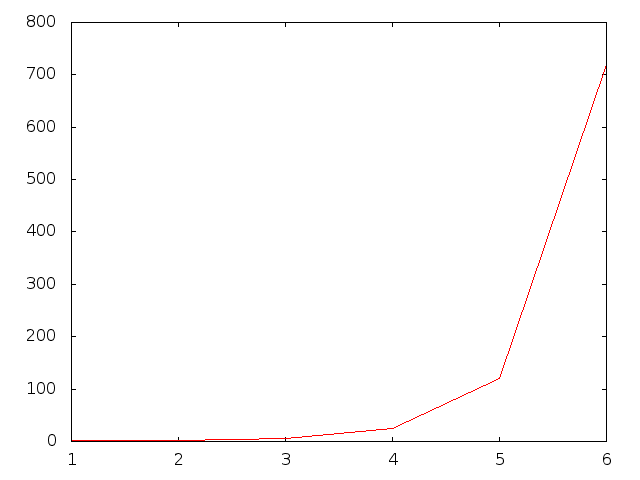
\includegraphics[width=0.60\textwidth,height=0.60\textheight,keepaspectratio]{testsPropios/graficoTest1.png}
\subsection{Tests de desambiguación}
	El código se encuentra en testsPropios/testBueno3.cod
	\lstinputlisting{testsPropios/testBueno3.cod}
	Salida:
	\lstinputlisting{testsPropios/salidaTest3.out}
	
	
	
	En este ejemplo vemos cómo resolvimos el problema de la desambiguación de los ifthenelse anidados. Nuestro enfoque es el mismo que el útilizado en lenguajes de programación conocidos como C. Podemos ver un ejemplo con el siguiente código:
		\lstinputlisting{testsPropios/pruebaIfThenElse.c}
	